\begin{figure*}[h]\centering
\makebox[\textwidth][c]{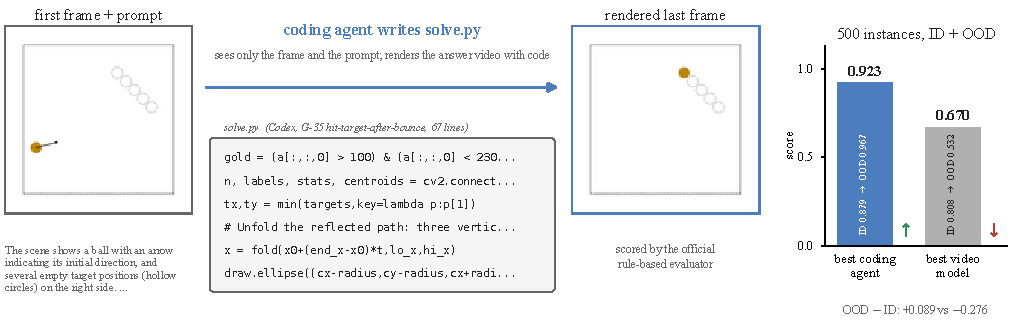
\includegraphics[width=0.9\textwidth]{figures/fig_teaser}}
\caption{\textbf{Solve vision with code.} A VBVR-Pro task hands the solver a first frame and a prompt and asks for the video in which the prompt is carried out; the official rule-based evaluator scores the result. \emph{Left:} the two inputs of one benchmark instance. \emph{Middle:} a coding agent answers by reading the frame, writing a program (six lines of the actual \texttt{solve.py} shown) and rendering the video with it; its last frame is on the right of the panel. It sees the same two inputs as a video model, produces the same output container, and is scored by the same evaluator. \emph{Right:} on VBVR-Pro-Bench the best coding agent scores 0.923 against 0.670 for the best video model, which was RL-trained on the benchmark's own in-domain task families; the agent's score rises from the in-domain to the out-of-domain half (0.879 to 0.967) while the trained video model's falls (0.808 to 0.532).}
\label{fig:teaser}
\end{figure*}

\begin{abstract}
VBVR-Pro asks whether generative models can reason natively in the visual medium: given a first frame and a prompt, a model must produce the video in which the task is carried out, and a rule-based evaluator scores the result \citep{vbvrpro2026}. Video generation models do poorly on it. The best, a Wan2.2 model RL-trained on the benchmark's own task families, scores 0.670 on VBVR-Pro-Bench. We keep the task, the inputs, the output container and the evaluator, and change only the medium of the answer: instead of denoising pixels, a coding agent writes a program that renders the video. The agent sees the first frame and the prompt inside a sandbox with no ground truth, no metadata and no image or video generation model, and it gets one attempt. Three closed-model agents reach 0.923 (Codex, gpt-6-astra), 0.894 (Claude Code, Fable 5.1) and 0.893 (Gemini CLI, Gemini 3.1 Pro): all three above 0.89 and 0.25 above the best video model. Their scores rise on the out-of-domain half of the benchmark, where every video model trained on it falls. Across 24 open-weight models the best reaches 0.572, above every video model except the RL-trained one, and the weakest fail by never using a tool at all. We release the agent harness and the per-instance evaluation results and run statistics behind every table; agent videos and run logs are available on request.
\end{abstract}
